\mySection{14.3 Wilcoxon Tests}
%-------------- start slide -------------------------------%{{{ 14.3
\begin{frame}
\begin{center}
	
\includegraphics[scale=0.15]{./Codes/Wilcoxon.png}
\end{center}
\end{frame}
%-------------- end slide -------------------------------%}}}
%-------------- start slide -------------------------------%{{{ 1
\begin{frame}[fragile]
	\frametitle{Testing $H_0:\mu=\mu_0$}
\begin{itemize}
	\item[Setup] Let $Y_1,\cdots, Y_n$ be a set of independent variables with pdfs $f_{Y_1}(y),\cdots, f_{Y_n}(y)$, respectively.
	\item[] Assume that $f_{Y_i}(y)$ are continuous and symmetric.
	\item[] Assume that all mean/median of $f_{Y_i}$ are equal, denoted by $\mu$.
	\bigskip
	\item[Test] $H_0:\mu=\mu_0$ vs. $H_1:\mu\ne \mu_0$.
	\mySeparateLine
	\bigskip
	\item[] \textcolor{yellow}{Wilcoxon signed rank static}
	\begin{align*}
		W = \sum_{k=1}^n  R_k\; \one_{\{Y_k>\mu_0\}}
	\end{align*}
	where $R_i$ denotes the rank (increasing and starting from 1) of
	\begin{align*}
		\left\{|Y_1-\mu_0|,|Y_2-\mu_0|,\cdots,|Y_n-\mu_0|\right\}
	\end{align*}
\end{itemize}
\end{frame}
%-------------- end slide -------------------------------%}}}
%-------------- start slide -------------------------------%{{{ 1
\begin{frame}[fragile]
\begin{center}
	\renewcommand{\arraystretch}{1.5}
	\begin{tabular}{c|ccc}
		$n$                     & 1                           & 2                           & 3                           \\ \hline
		$y_n$                   & 4.2                         & 6.1                         & 2.0                         \\
    $y_n-3.0$               & 1.2                         & 3.1                         & -1.0                        \\
    $\left|y_n-3.0\right|$  & 1.2                         & 3.1                         & 1.0                         \\
		$r_n$                   & \textcolor{magenta}{2}      & \textcolor{magenta}{3}      & \textcolor{magenta}{1}      \\
		$\one_{\{y_n>3.0\}}$    & \textcolor{cyan}{1}         & \textcolor{cyan}{1}         & \textcolor{cyan}{0}         \\ [1em]
		$r_n\one_{\{y_n>3.0\}}$ & \textcolor{yellow}{$u_2=2$} & \textcolor{yellow}{$u_3=3$} & \textcolor{yellow}{$u_1=0$} \\
	\end{tabular}
\end{center}
\bigskip
\[\Downarrow\]
\begin{align*}
	w= \textcolor{magenta}{2}\times \textcolor{cyan}{1} + \textcolor{magenta}{3} \times \textcolor{cyan}{1} + \textcolor{magenta}{1} \times \textcolor{cyan}{0} = 5.
\end{align*}
\end{frame}
%-------------- end slide -------------------------------%}}}
%-------------- start slide -------------------------------%{{{ 1
\begin{frame}[fragile]

	\begin{center}
	Let $\{y_1,\cdots,y_n\}$  be For a sample of size $n$.
	\end{center}
\vfill
{\bf Some observations:}
\bigskip
\begin{itemize}
	\item $r_i$ takes values in $\{1,2,\cdots, n\}$.
		\bigskip
	\item $w_i$ takes values in $\left\{0,1,2,\cdots, \frac{n(n+1)}{2}\right\}$ with $1+2+\cdots + n = \frac{n(n+1)}{2}$.
		\bigskip
	\item $W$ is a discrete random variable:
		\bigskip

		\begin{center}
		\renewcommand{\arraystretch}{1.5}
		\begin{tabular}{|c|c|c|c|c|}
			$w$         & 0 & 1 & $\cdots$ & $\frac{n(n+1)}{2}$ \\ \hline
			$\bbP(W=w)$ &   &   &          &                    \\
		\end{tabular}
		\end{center}
\end{itemize}
\end{frame}
%-------------- end slide -------------------------------%}}}
%-------------- start slide -------------------------------%{{{ 1
\begin{frame}[fragile]
\begin{itemize}
	\item[Theorem] Under the above setup and under $H_0$,
	\begin{align*}
		p_W(w) = \bbP(W=w) = \frac{c(w)}{2^n},
	\end{align*}
	where $c(w)$ is the coefficient of  $e^{wt}$ in the expansion of
	 \begin{align*}
		\prod_{k=1}^n \left(1+e^{kt}\right).
	\end{align*}
	\bigskip
	\item[Proof] Under $H_0$,  $W=\sum_{k=1}^n U_k$ with follow the following distribution
	\begin{align*}
		U_k =
		\begin{cases}
			0& \text{with probability $1/2$}\\
			k& \text{with probability $1/2$}.
		\end{cases}
	\end{align*}
	\item[] Then
	\begin{align*}
		M_W(t) = \prod_{k=1}^n M_{U_k}(t) = \prod_{k=1}^n\E\left(e^{U_kt}\right) = \prod_{k=1}^n \left(\frac{1}{2} +\frac{1}{2}e^{kt}\right).
	\end{align*}
\end{itemize}
\end{frame}
%-------------- end slide -------------------------------%}}}
%-------------- start slide -------------------------------%{{{ 1
\begin{frame}[fragile]
\begin{itemize}
	\item[] Hence, we have
	\begin{align*}
		M_W(t) =\frac{1}{2^n}\prod_{k=1}^n\left(1+e^{kt}\right).
	\end{align*}
	\item[] On the other hand,
	\begin{align*}
		M_W(t) = \E\left(e^{Wt}\right) = \sum_{w=0}^{\frac{n(n+1)}{2}} e^{wt} p_W(w)
	\end{align*}
	\item[] Equating the above two expressions, namely,
	\begin{align*}
		\frac{1}{2^n}\prod_{k=1}^n\left(1+e^{kt}\right) = \sum_{w=0}^{\frac{n(n+1)}{2}} e^{wt} p_W(w),
	\end{align*}
	proves the theorem.\myQED
\end{itemize}
\end{frame}
%-------------- end slide -------------------------------%}}}
%-------------- start slide -------------------------------%{{{ 1
\begin{frame}[fragile]
\begin{itemize}
	\item[E.g.] Find the pdf of $W$ when $n=2$ and $4$.
	\bigskip

	\item[Sol.] When $n=2$,
	 \begin{align*}
		M_W(t) & = \frac{1}{2^2} \left(1+e^t\right)\left(1+e^{2t}\right)\\
           & = \frac{1}{2^2} (1+e^t+e^{2t}+e^{3t}).
	\end{align*}
	Hence,
	\begin{center}
		\renewcommand{\arraystretch}{1.5}
		\begin{tabular}{|c|c|c|c|c|}
			$w$      & 0 & 1 & 2 & 3 \\\hline
			$p_W(w)$ & $1/4$ & $1/4$ & $1/4$ & $1/4$
		\end{tabular}
	\end{center}
\end{itemize}
\end{frame}
%-------------- end slide -------------------------------%}}}
%-------------- start slide -------------------------------%{{{ 1
\begin{frame}[fragile]
\begin{itemize}
	\item[] When $n=4$,
	 \begin{align*}
		M_W(t) & = \frac{1}{2^4} \left(1+e^t\right)\left(1+e^{2t}\right)\left(1+e^{3t}\right)\left(1+e^{4t}\right)\\
           & = \frac{1}{16} \left( e^{10t} + e^{9t} + e^{8t} + 2e^{7t} + 2e^{6t} + 2e^{5t} + 2e^{4t} + 2e^{3t} + e^{2t} + e^t + 1\right).
	\end{align*}
	Hence,
	\begin{center}
		\renewcommand{\arraystretch}{1.5}
		\begin{tabular}{|c|c|c|c|c|c|c|c|c|c|c|c|}
			$w$      & 0              & 1              & 2              & 3              & 4              & 5              & 6              & 7              & 8              & 9              & 10             \\ \hline \bigskip
			$p_W(w)$ & $\frac{1}{16}$ & $\frac{1}{16}$ & $\frac{1}{16}$ & $\frac{2}{16}$ & $\frac{2}{16}$ & $\frac{2}{16}$ & $\frac{2}{16}$ & $\frac{2}{16}$ & $\frac{1}{16}$ & $\frac{1}{16}$ & $\frac{1}{16}$ \\
		\end{tabular}
	\end{center}
	\myQED
\end{itemize}
\vfill
\mySeparateLine
\begin{lstlisting}
sage: var('k,t')
(k, t)
sage: product(1+e^(k*t),k,1,4)
e^(10*t) + e^(9*t) + e^(8*t) + 2*e^(7*t) + 2*e^(6*t) + 2*e^(5*t) + 2*e^(4*t) + 2*e^(3*t) + e^(2*t) + e^t + 1
\end{lstlisting}
%
% product(1+e^(k*t),k,1,10)
%
% product(1+e^(k*t),k,1,10)/2^( 10 )
%
%
% 2*( 1/512 + 1/512 + 3/1024 )
%
% N(_)
%
%
% 2*( 1/512 + 1/512 + 6/1024 )
% N(_)
%
\end{frame}
%-------------- end slide -------------------------------%}}}
%-------------- start slide -------------------------------%{{{ 1
\begin{frame}[fragile]
\begin{itemize}
	\item[E.g.] Shark studies:
	\begin{center}
		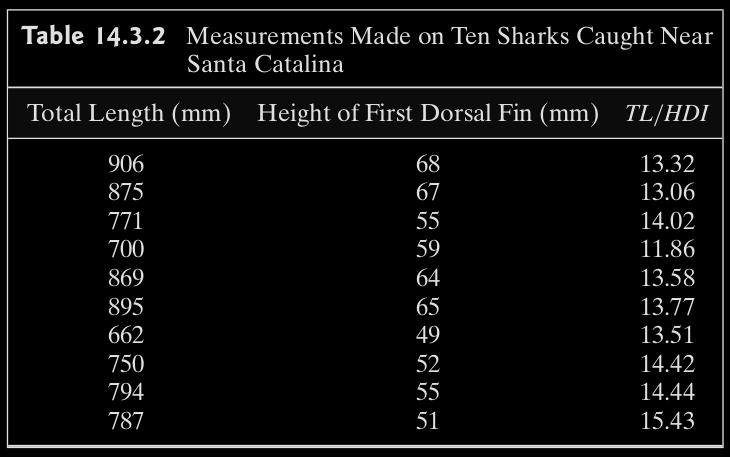
\includegraphics[scale=0.25]{Codes/Table14-3-2.png}
	\end{center}
	\item[] Past data show that the true average $TL/HDI$ ratio should be $14.60$.
	\item[] Let $Y_i=TL/HDI$.
	\item[] Does the data support the above claim, namely, test
	\begin{align*}
		H_0:\mu=14.60 \quad \text{vs.} \quad H_1:\mu\ne 14.60.
	\end{align*}
	\item[] Set $\alpha=0.05$.
\end{itemize}
\end{frame}
%-------------- end slide -------------------------------%}}}
%-------------- start slide -------------------------------%{{{ 1
\begin{frame}[fragile]
\begin{itemize}
	\item[Sol.] Computing the Wilcoxon signed rank statistics:
	\begin{center}
		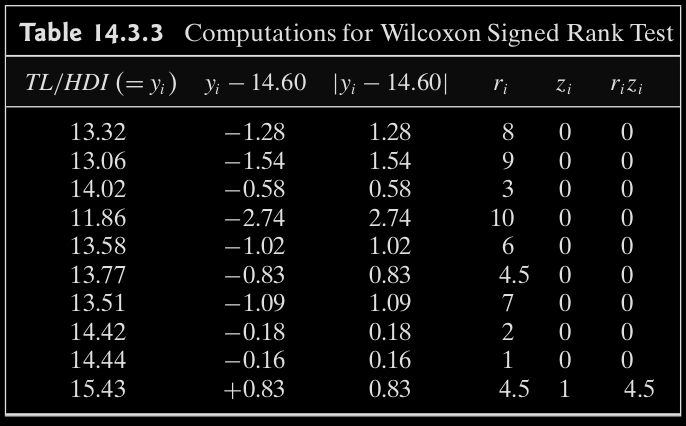
\includegraphics[scale=0.25]{Codes/Table14-3-3.png}
	\end{center}
	\item[] Hence, $w=4.5$.
	\item[] Now check the table to find the critical region:
	\begin{align*}
		C = \{w: w\le 8\quad \text{or}\quad w\ge 47\}.
	\end{align*}
	\item[] Conclusion: Rejection!\myQED
\end{itemize}
\end{frame}
%-------------- end slide -------------------------------%}}}
%-------------- start slide -------------------------------%{{{ 1
\begin{frame}[fragile]
\lstset{language=R}
\begin{lstlisting}
> x <- c(13.32, 13.06, 14.02, 11.86, 13.58, 13,77, 13.51, 14.42, 14.44, 15.43)
> wilcox.test(x, mu = 14.60, alternative = "two.sided")

        Wilcoxon signed rank exact test

data:  x
V = 15, p-value = 0.123
alternative hypothesis: true location is not equal to 14.6
\end{lstlisting}
%
% x <- c(13.32, 13.06, 14.02, 11.86, 13.58, 13,77, 13.51, 14.42, 14.44, 15.43)
%
% wilcox.test(x, mu = 14.60, alternative = "two.sided")
%
\end{frame}
%-------------- end slide -------------------------------%}}}
%-------------- start slide -------------------------------%{{{ 1
\begin{frame}[fragile]
	\frametitle{Large-sample Wilcoxon Signed Rank Test}
\begin{itemize}
	\item[Theorem] Under the same setup and $H_0$, we have
	\begin{align*}
		\E(W) = \frac{n(n+1)}{4}\quad\text{and}\quad \Var(W)=\frac{n(n+1)(2n+1)}{24}.
	\end{align*}
	\bigskip
	\item[Proof.]
	\begin{align*}
		\E(W) & = \E\left(\sum_{k=1}^n U_k\right) = \sum_{k=1}^n \left(0\cdot \frac{1}{2}+k\cdot \frac{1}{2}\right)\\
          & = \sum_{k=1}^n \frac{k}{2} = \frac{n(n+1)}{4}.
	\end{align*}
	\begin{align*}
		\Var(W) & = \Var\left(\sum_{k=1}^n U_k\right) = \sum_{k=1}^n \Var(U_k) = \sum_{k=1}^n \left[ \E(U_k^2) - \E(U_k)^2\right] \\
            & = \sum_{k=1}^n \left[ \frac{k^2}{2} - \left(\frac{k}{2}\right)^2\right] = \sum_{k=1}^n \frac{k^2}{4} = \frac{1}{4} \frac{n(n+1)(2n+1)}{6}
	\end{align*}
	\myQED
\end{itemize}
\end{frame}
%-------------- end slide -------------------------------%}}}
%-------------- start slide -------------------------------%{{{ 1
\begin{frame}[fragile]
\begin{itemize}
	\item[Hence] when $n$ is large (usually $n\ge 12$),
	\begin{align*}
		\frac{W-\E(W)}{\sqrt{\Var(W)}} = \frac{W-[n(n+1)]/4}{\sqrt{[n(n+1)(2n+1)]/24}} \quad \stackrel{approx}{\sim}\quad N(0,1).
	\end{align*}
\end{itemize}
\[\Downarrow\]
\begin{center}
	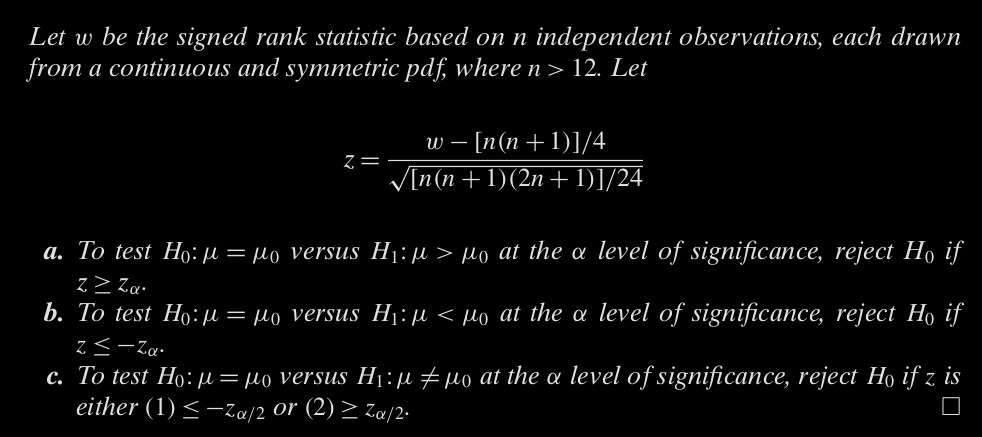
\includegraphics[scale=0.31]{Codes/Theorem14-3-3.png}
\end{center}
\end{frame}
%-------------- end slide -------------------------------%}}}
%-------------- start slide -------------------------------%{{{ 1
\begin{frame}[fragile]
\frametitle{The Wilcoxon Rank Sum Test \\ \small -- Nonparametric counterpart of the pooled two-sample t-test}
 \begin{itemize}
 	\item[Setup] Let $x_1,\cdots, x_n$ and  $y_{n+1},\cdots, y_{n+m}$ be two independent random samples from $f_X(x)$ and  $f_Y(y)$, respectively.
	\item[] Assume that  $f_X(x)$ and  $f_Y(y)$ are the same except for a possible shift in location.
	\bigskip
	\item[Test] $H_0:\mu_x=\mu_y$ vs. ...
	\bigskip
	\item[] \textcolor{magenta}{Test statistic}
	\begin{align*}
		W = \sum_{k=1}^{n+m} R_i Z_i
	\end{align*}
	where $R_i$ is the rank (starting from the lowest with rank 1) and
	 \begin{align*}
		Z_i =
		\begin{cases}
			1 &  \text{the ith entry comes from $f_X(x)$}\\
			0 &  \text{the ith entry comes from $f_Y(y)$}.
		\end{cases}
	\end{align*}
\end{itemize}
% \begin{itemize}
% 	\item[Remark] Wilcoxon Signed Rank Test can be naturally applied to paired data and can be used to study two-sample test.
% \end{itemize}
\end{frame}
%-------------- end slide -------------------------------%}}}
%-------------- start slide -------------------------------%{{{ 1
\begin{frame}[fragile]
\begin{itemize}
	\item[Theorem] Under the above setup and under $H_0$,
	 \begin{align*}
		\E[ W ]  = \frac{n(n+m+1)}{2}\quad \text{and}\quad \Var(W) = \frac{nm(n+m+1)}{12}.
	\end{align*}
		\bigskip
	\item[Hence] when sample sizes are large, namely, $n,m>10$,
		 \bigskip
	\begin{align*}
		\frac{W-\E(W)}{\sqrt{\Var(W)}} = \frac{W-[n(n+m+1)]/2}{\sqrt{[nm(n+m+1)]/12}} \quad \stackrel{approx}{\sim}\quad N(0,1).
	\end{align*}
\end{itemize}
\end{frame}
%-------------- end slide -------------------------------%}}}
%-------------- start slide -------------------------------%{{{ 1
\begin{frame}[fragile]
\begin{itemize}
	\item[E.g.] Baseball ...
\begin{center}
	Test if $H_0:\mu_X=\mu_Y$ vs. $H_0:\mu_X\ne\mu_Y$
	\bigskip

	\begin{center}
		\begin{tikzpicture}[scale=1, transform shape]
			\node (fig) at (0,0) {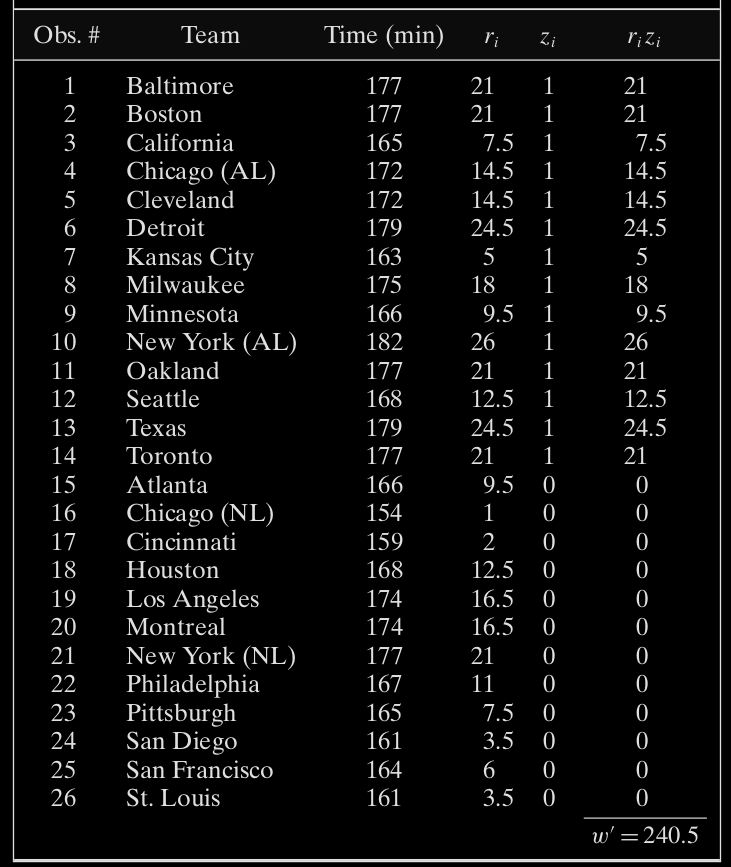
\includegraphics[scale=0.25]{./Codes/Table14-3-7.png}};
			\pause
			\draw[red] (-3,-0.33) rectangle ++(6,+3) node [right] {Group $X$};
			\pause
			\draw[red] (-3,-0.36) rectangle ++(6,-3) node [right] {Group $Y$};
		\end{tikzpicture}
	\end{center}
\end{center}
\end{itemize}
\end{frame}
%-------------- end slide -------------------------------%}}}
%-------------- start slide -------------------------------%{{{ 1
\begin{frame}[fragile]
\begin{itemize}
	\item[] In this case, $n=14$,  $m=12$,  $w=240.5$.
	\begin{gather*}
		\E(W) = \frac{14(14+12+1)}{2} = 189,\\
		\Var(W) = \frac{14\times 12 \times (14+12+1)}{12} = 378.
	\end{gather*}
	\item[] Hence, the approximate z-score is
	\begin{align*}
		z = \frac{w-\E(W)}{\sqrt{\Var(W)}} = \frac{240.5-189}{\sqrt{378}} = 2.65.
	\end{align*}
	\item[]...\myQED
\end{itemize}
\end{frame}
%-------------- end slide -------------------------------%}}}
